\documentclass[12pt,a4paper]{scrartcl}
\usepackage[utf8]{inputenc}
\usepackage{amsmath}
\usepackage{amsfonts}
\usepackage{amssymb}
\usepackage{graphicx}

\usepackage[bottom = 1in, left = 0.5in, right = 0.5in, top = 1in]{geometry}

\usepackage[english]{babel}
\usepackage[autostyle]{csquotes}
\usepackage{mathptmx}

\usepackage[labelfont=bf]{caption}

\usepackage[default, scale=0.95]{opensans}

\usepackage[T1]{fontenc}

\usepackage{fixltx2e}

\title{Figures}
\date{}

\begin{document}
\maketitle

\begin{figure}[h]
	\centering
	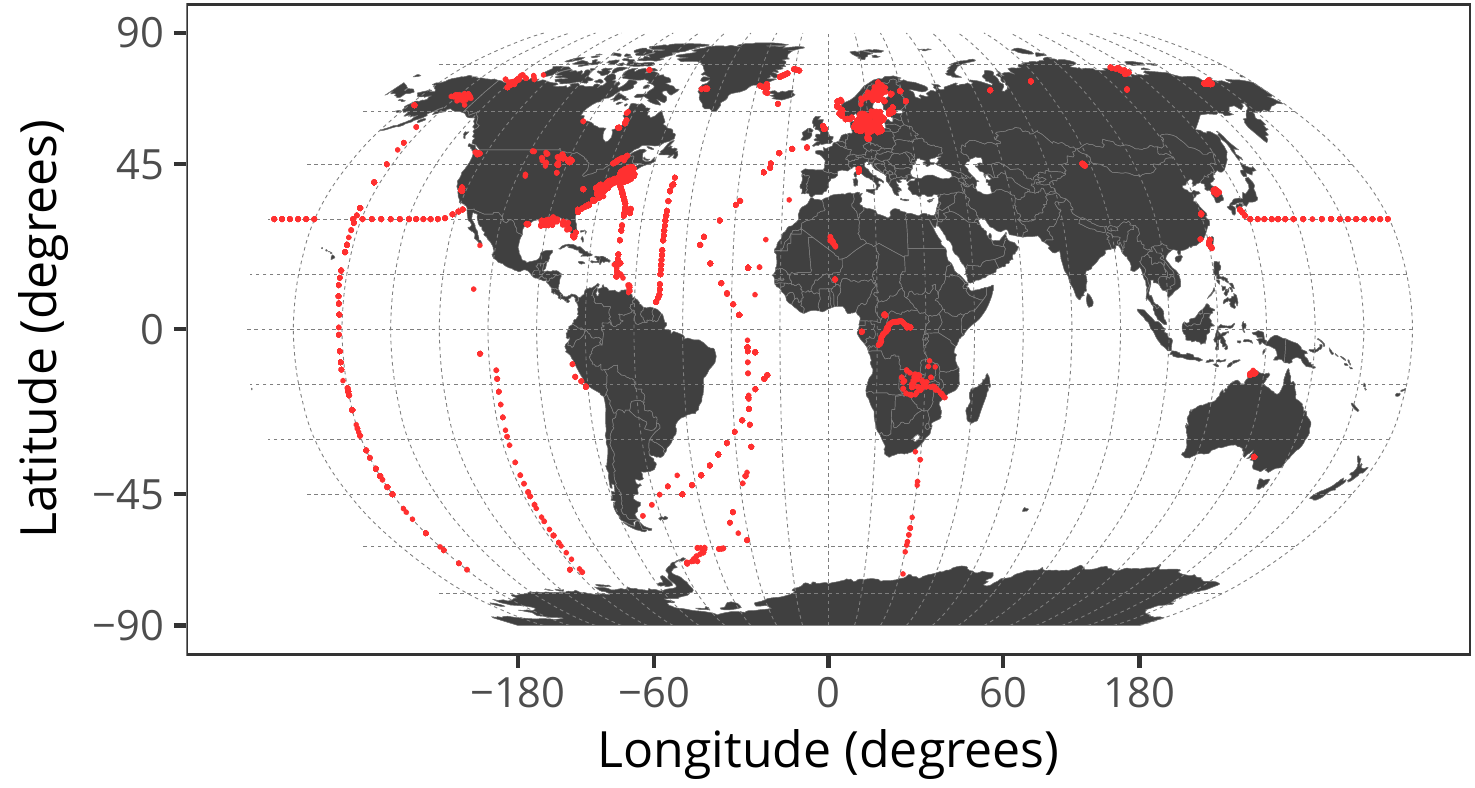
\includegraphics[scale = 1.25]{../../graphs/fig1}
	\caption{World map showing the spatial distribution of the observations extracted from the literature ($n = 12 808$ different sampling locations).}
\end{figure}

\clearpage
\newpage

\begin{figure}[h]
	\centering
	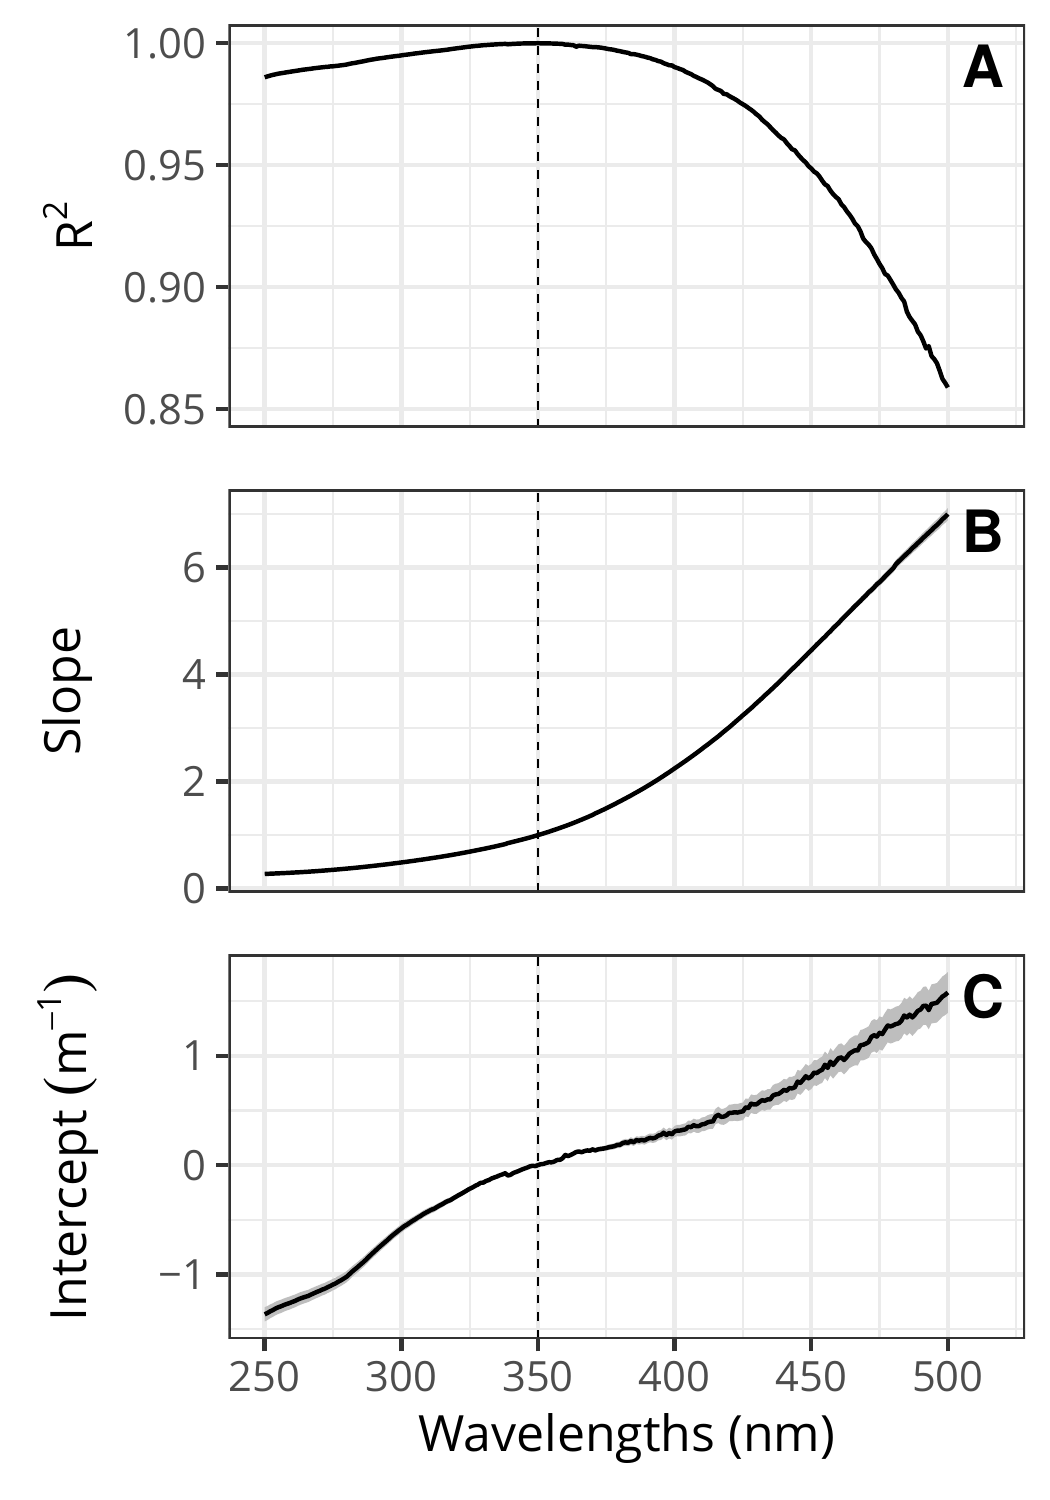
\includegraphics[scale = 1]{../../graphs/fig2}
	\caption{Determination coefficient ($R^2$) showing the goodness of the linear fit between DOC and absorption coefficients measured at different wavelengths for freshwater ($n = 797$), coastal ($n = 995$) and ocean ecosystems ($n = 442$). Vertical dashed line represents the chosen wavelength of 350 nm used to explore the relationship between DOC and $a\textsubscript{CDOM}(350)$ (see Fig. 5).}
\end{figure}

\clearpage
\newpage

\begin{figure}[h]
	\centering
	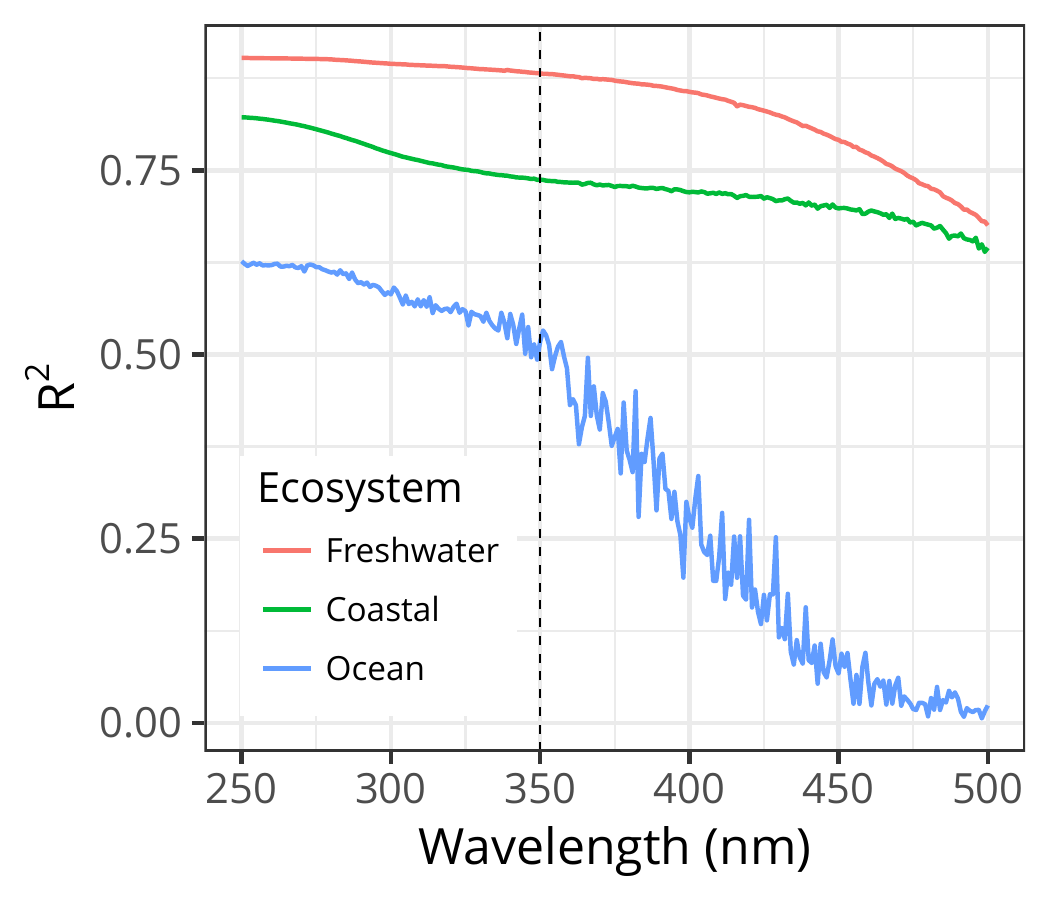
\includegraphics[scale = 0.8]{../../graphs/fig3}
	\caption{Boxplots showing the distribution of (\textbf{A}) absorption coefficients at 350 nm ($a_{CDOM}(350)$), (\textbf{B}) dissolved organic carbon (DOC) and (\textbf{C}) the specific ultra-violet absorbance at 350 nm (SUVA\textsubscript{350}). Y-axis are log-transformed given the wide ranges spanned by the data. Numbers on the bottom of each panel represent the coefficient of variations (CV) as a standardized measure of the variability associated to each ecosystems. Note that the values of the specific absorption coefficient ($a^*$) are also presented on the right y-axis.}
\end{figure}

\clearpage
\newpage

\begin{figure}[h]
	\centering
	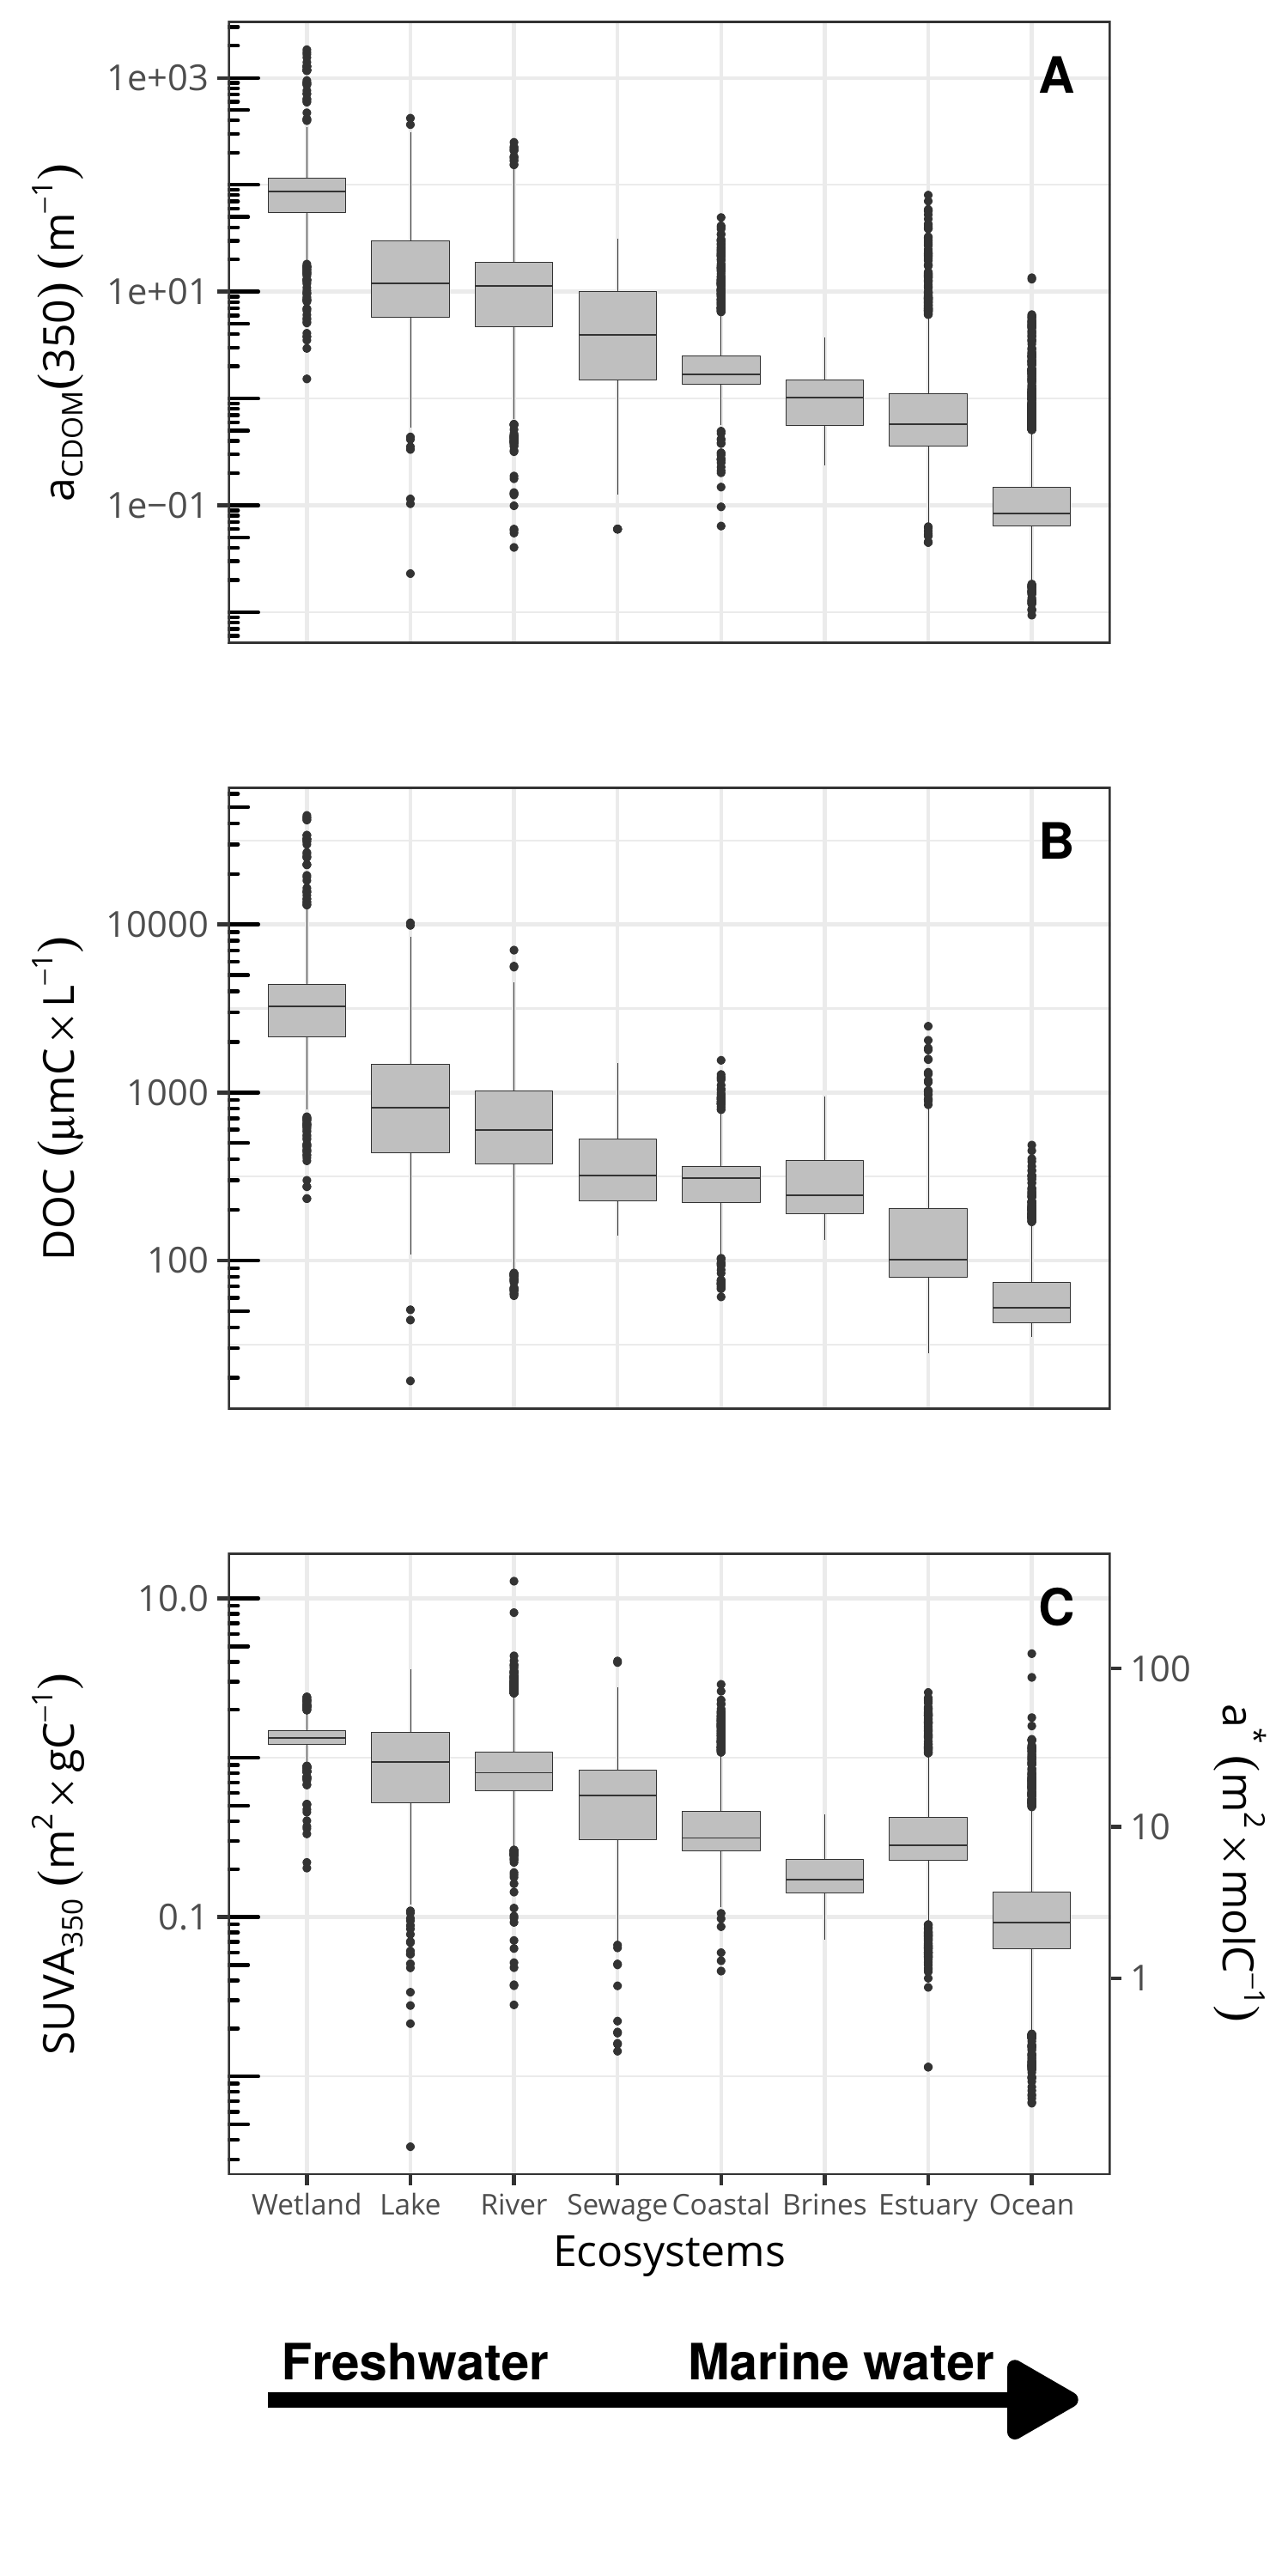
\includegraphics[scale = 1]{../../graphs/fig4}
	\caption{(\textbf{A}) Global relationship between absorption at 350 nm a\textsubscript{CDOM}(350) and dissolved organic carbon. The blue line is the fitted values of a linear model $y~=~\log(x)$, $R^2~=~0.92$, $p~<~0.00001$, $n~=~12808$. (\textbf{B}) Barplot showing the determination coefficient ($R^2$) of the linear relationships between a\textsubscript{CDOM}(350) and DOC by ecosystems. The dashed horizontal line represents the average of $R^2$.}
\end{figure}

\clearpage
\newpage

\begin{figure}[h]
	\centering
	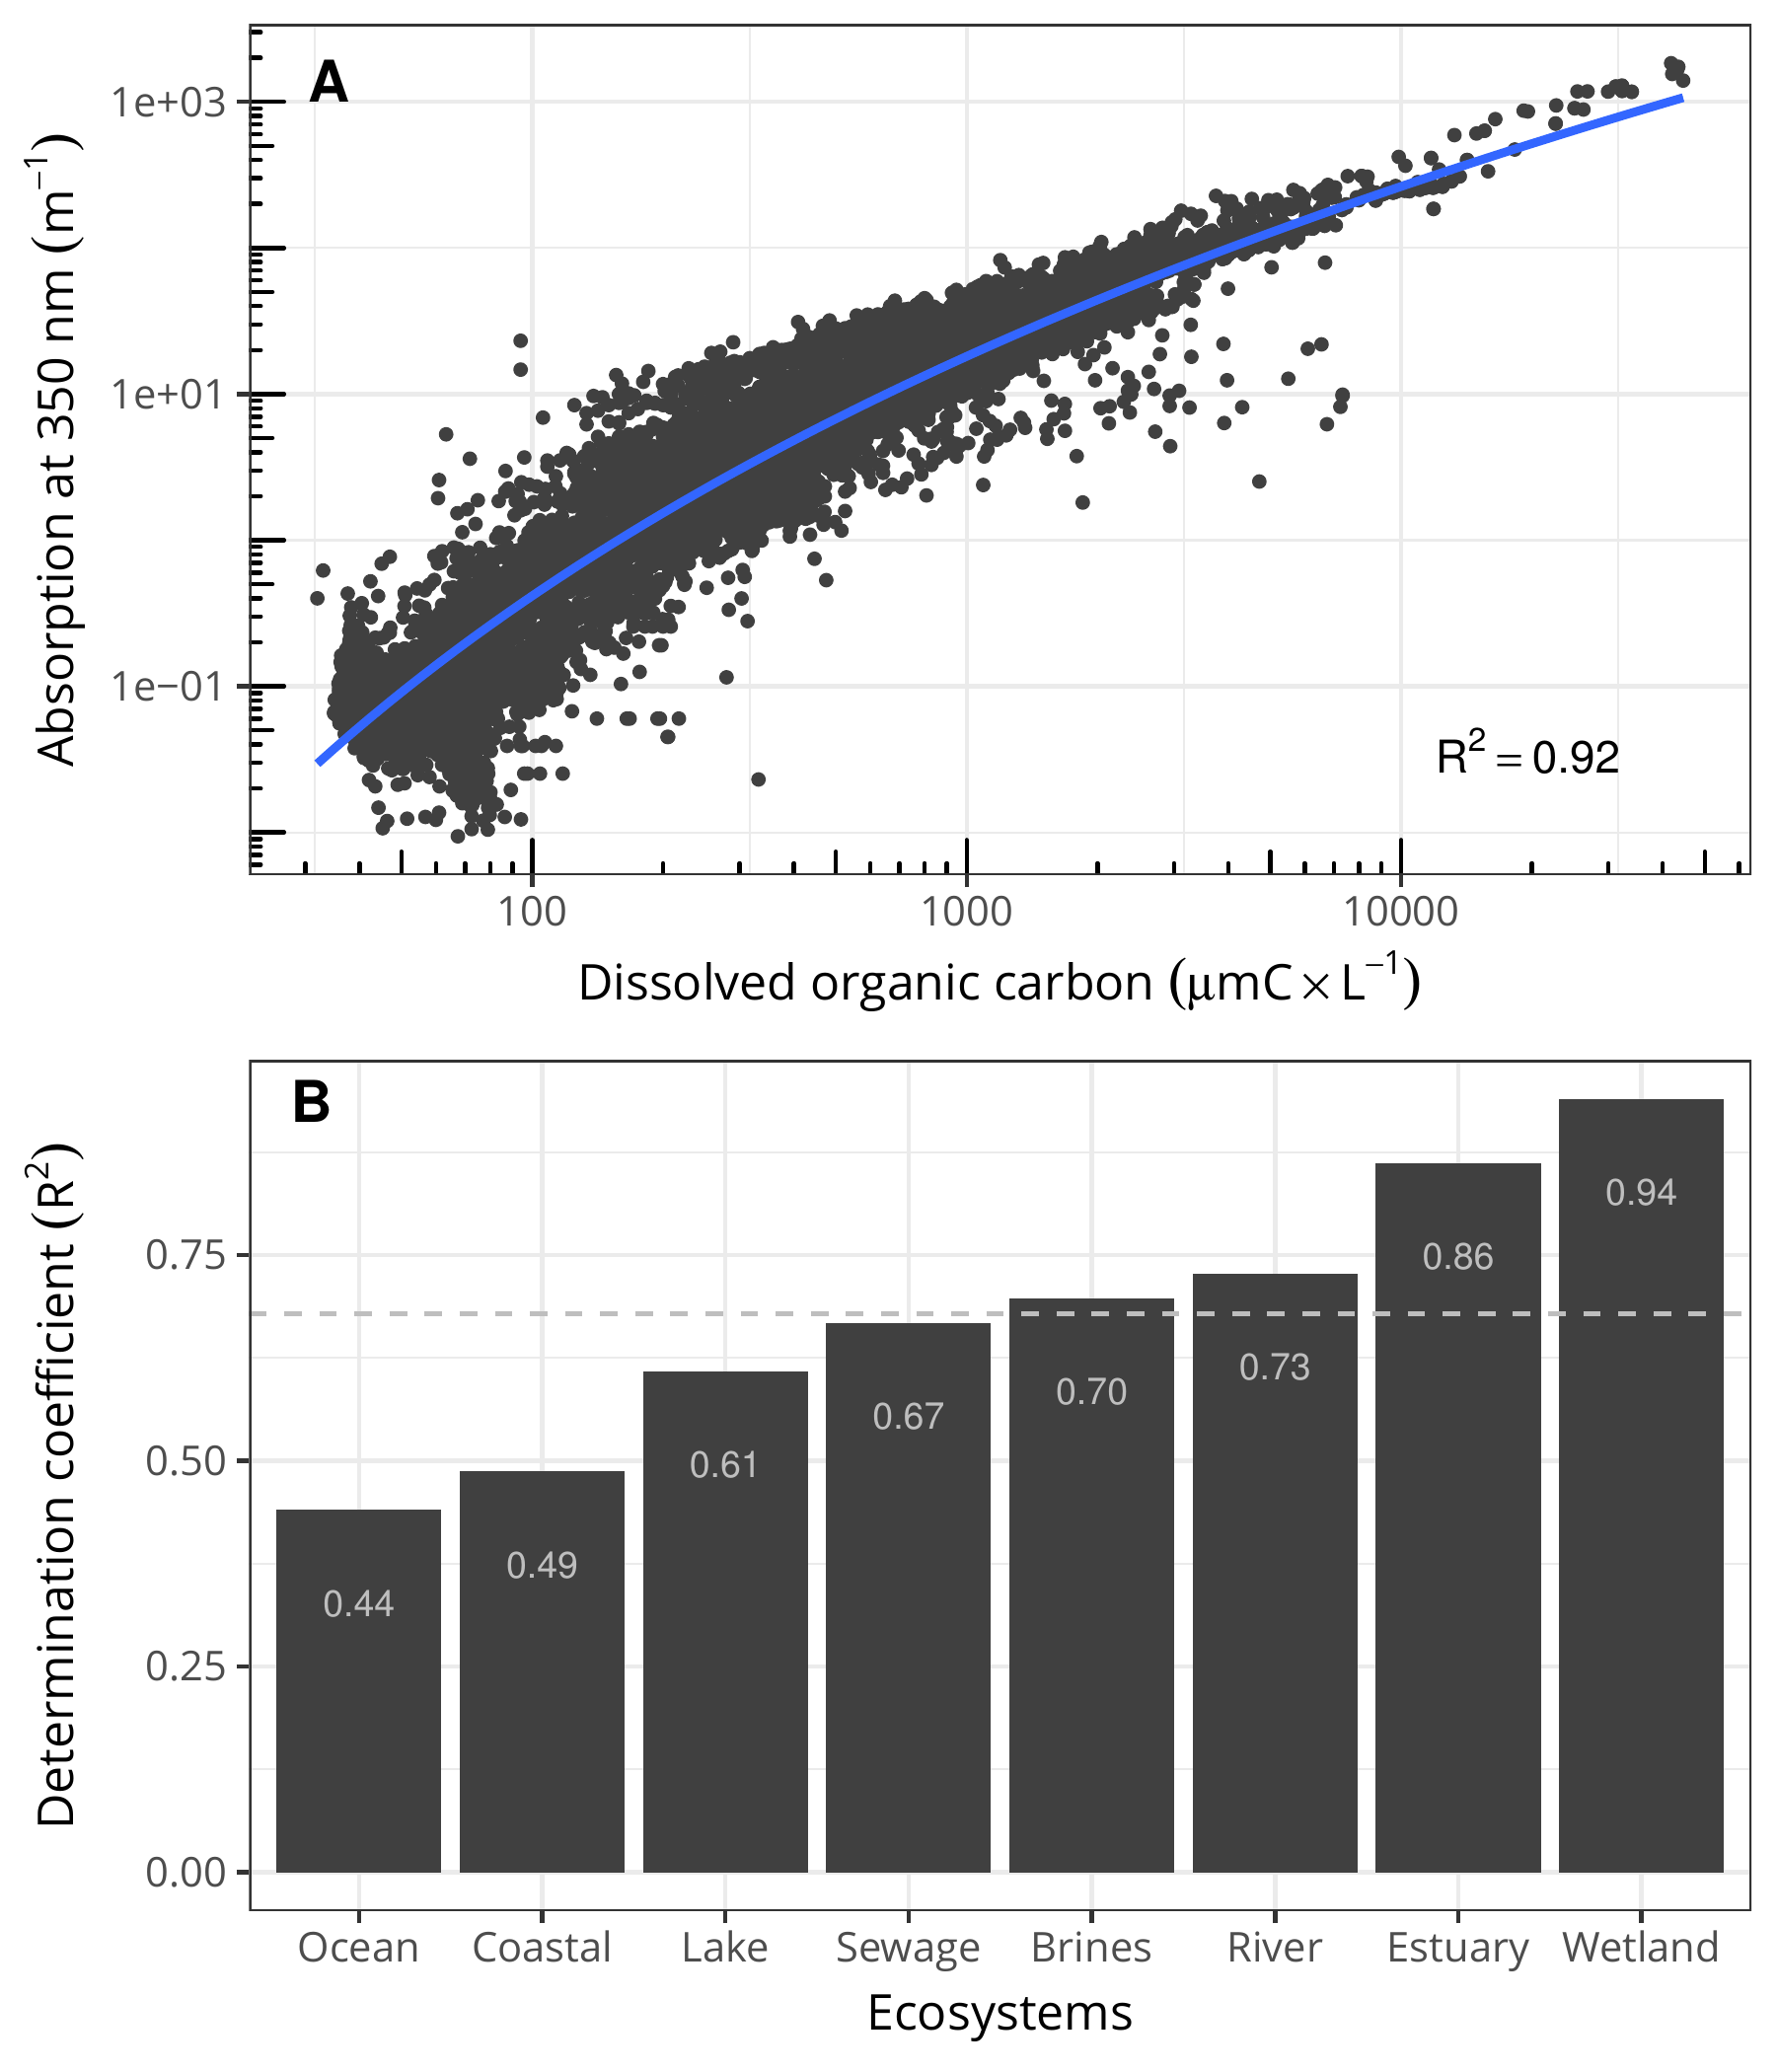
\includegraphics[scale = 1]{../../graphs/fig5}
	\caption{Averaged SUVA\textsubscript{254} calculated using observations from river and ocean ecosystems as a function of the distance to the closest shoreline (vertical error bars are the standard errors around the calculated mean). Positive distances represent inland samples (rivers) whereas negative distances represent oceanic samples. The blue line represents the segmentation analysis performed on the linear relationship between SUVA\textsubscript{254} and distance ($R^2~=~0.95, p~<~0.00001$). Dashed vertical line represents the identified breakpoint at 370 $\pm$ 102 km (shaded area) away from the shoreline toward the ocean.  Note that the values of the specific absorption coefficient ($a^*$) are also presented on the right y-axis.}

\end{figure}

\clearpage
\newpage

\begin{figure}[h]
	\centering
	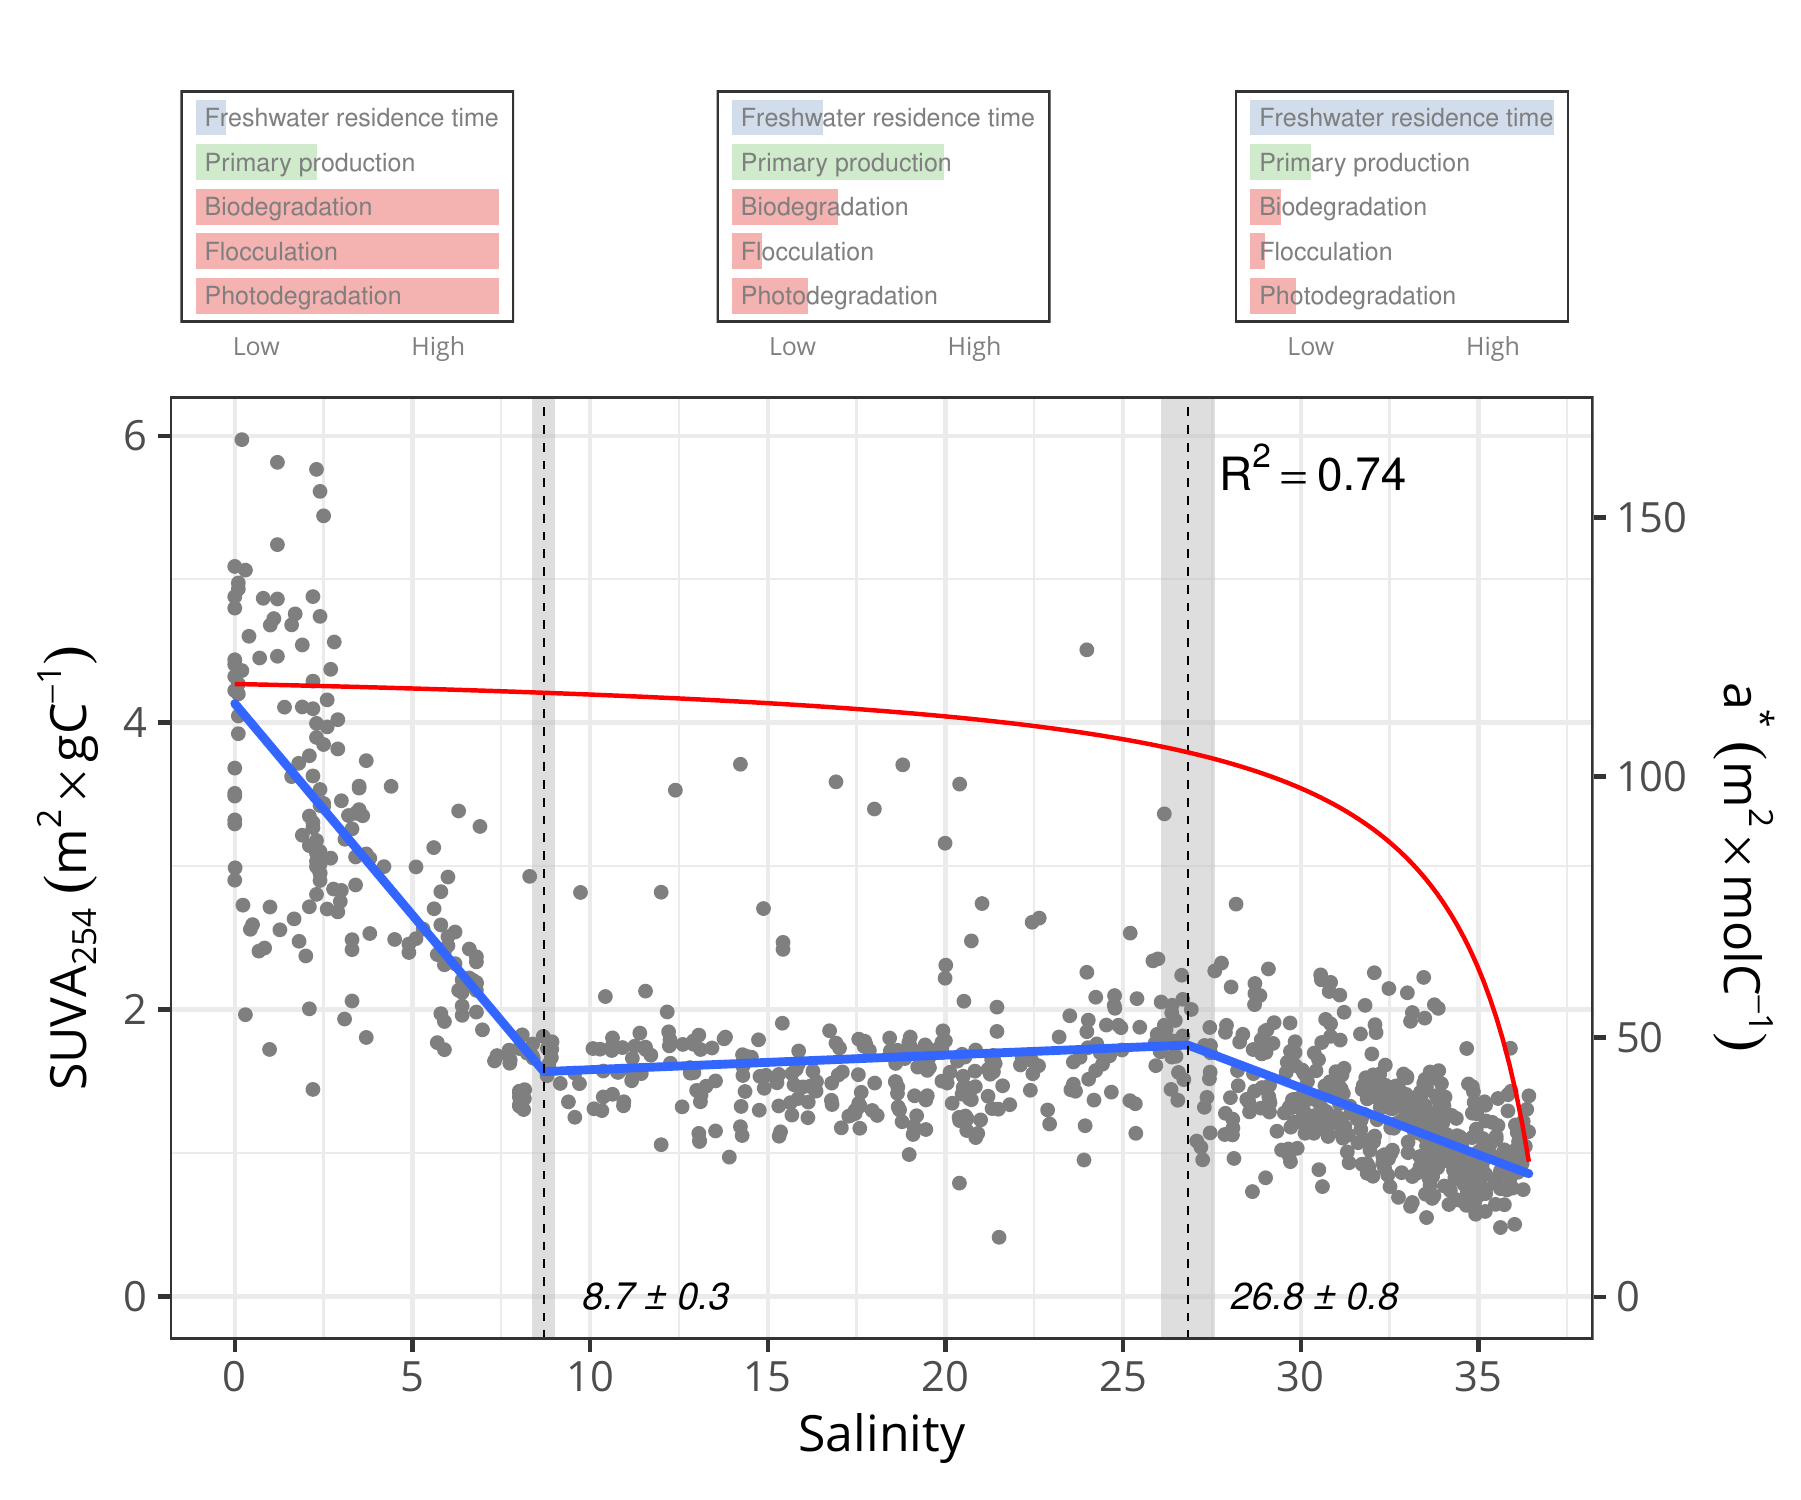
\includegraphics[scale = 1]{../../graphs/fig6}
	\caption{Segmentation analysis performed on the linear relationship between SUVA\textsubscript{254} and salinity ($R^2~=~0.7, p~<~0.00001, n~=~1080$). Dashed vertical lines represent the identified breakpoints at salinity 8.5 and 28.4 (shaded areas are standard errors). Conceptual plots above the identified segments represent the hypothesized processes driving SUVA\textsubscript{254}. The gray diagonal dashed-line indicates the hypothetical conservative mixing line between SUVA\textsubscript{254} and salinity.  Note that the values of the specific absorption coefficient ($a^*$) are also presented on the right y-axis.}
\end{figure}

\clearpage
\newpage

\begin{figure}[h]
	\centering
	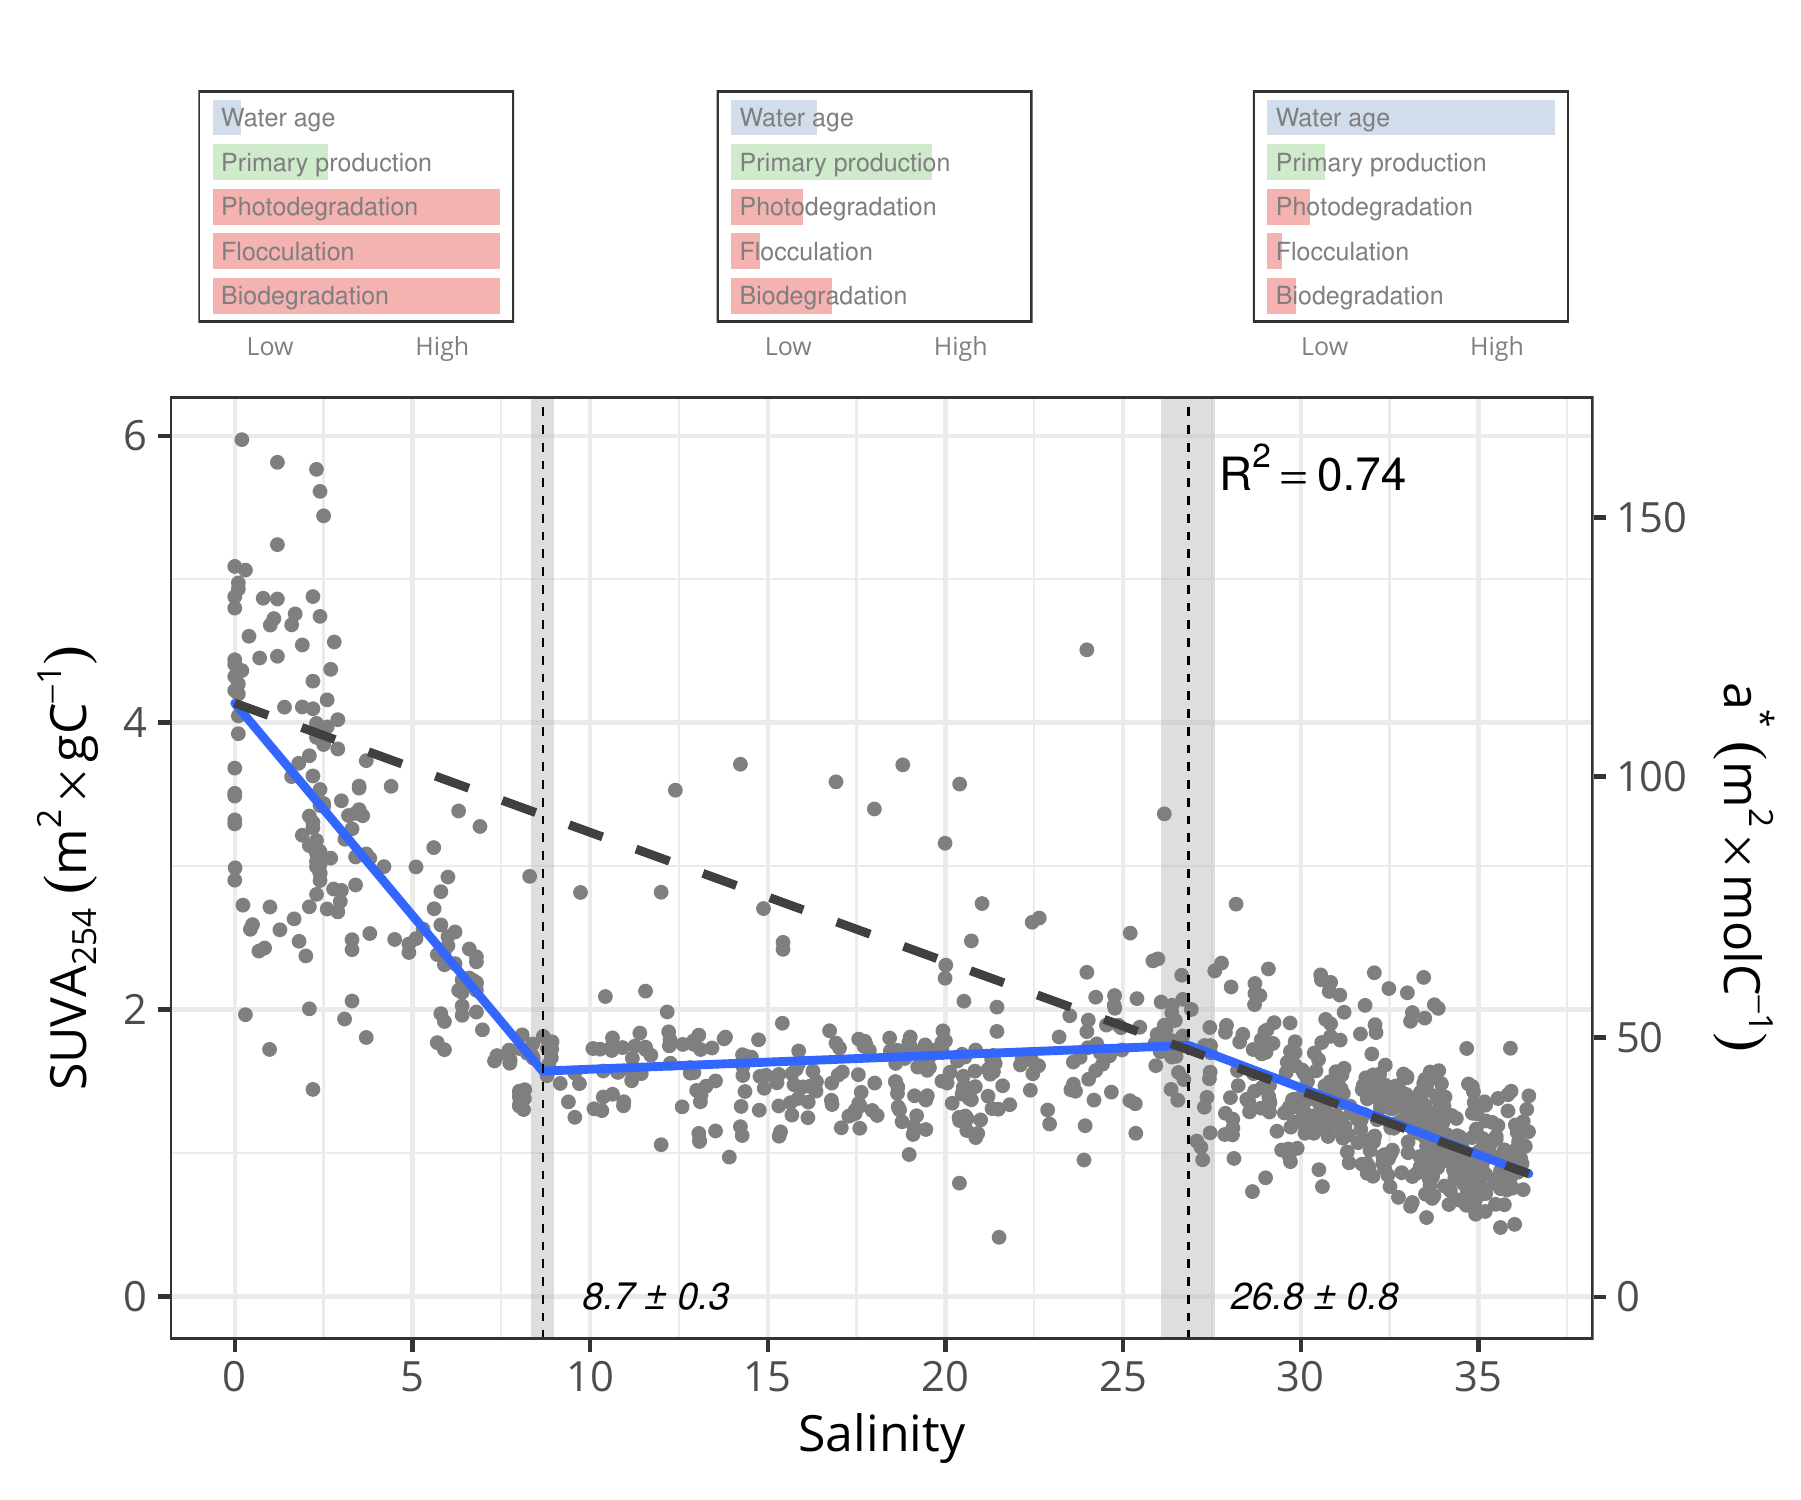
\includegraphics[scale = 1]{../../graphs/fig7}
	\caption{Spectral slope curve (S\textsubscript{$\lambda$}) calculated on averaged absorption spectra on freshwater and marine ecosystems using a 21 nm wavelength interval. $R^2$ for the calculated fit is indicated by color for each point on the spectrum.}
\end{figure}

\end{document}
